\documentclass[a4paper,12pt]{article}
\usepackage{graphicx} % Required for inserting images
\usepackage{fancyvrb}
\usepackage{xcolor}
\usepackage{tikz, tcolorbox}
\usepackage[utf8]{inputenc}
\usepackage[spanish]{babel}
\usepackage{amsmath, amssymb}
\usepackage{hyperref}
\usepackage{listings}
\usepackage{geometry}
\usepackage{float}
\title {
\includegraphics[width=0.4\textwidth]{Ing_Uni.jpg}\\[2ex]{\textbf{Informe Proyecto\\ Restaurante}\\[1.5ex] Programacion II\\[20ex]}}
\author{Diego Hernandez, Benjamin Soto, Eduardo Necul}
\date{Octubre 2025}

\lstset{
    backgroundcolor=\color{gray!10},
    basicstyle=\ttfamily\footnotesize,
    frame=single,
    breaklines=true,
    keywordstyle=\color{blue},
    commentstyle=\color{green!50!black},
    stringstyle=\color{orange},
    showstringspaces=false
}

\begin{document}

\maketitle
\newpage

\section{Introduccion}

Se nos hizo entrega un codigo base para la funcion de un restaurante incompleto, en cual nosotros debemos encargarnos de completarlo y refinarlo con la forma de programar \textbf{POO} (programacion orientada a objetos), sin salirnos de las casillas del esqueleto inicial. Ademas nos preucuparemos de de explicar cada cambio aplicado al codigo, que utilidad le dimos a las funciones vacias y el diagrama de clases en base a este.

\section{Cambios y implementaciones}

Apartado donde nos centraremos en explicar que modificamos en el codigo para su mejor compresion y funcionalidad.

\subsection{Cambios de variable o definiciones}

\begin{lstlisting}[language=Python, caption={Cambios de definiciones o variables}, frame=single]
def actualizar_treeview => def actualizar_treeview_stock
def configurar_pestana1 => def configurar_pestana_stock
def configurar_pestana2 => def configurar_pestana_pedido
def configurar_pestana3 => def configurar_pestana_CSV
self.treeview_menu => self.treeview_pedido
tarjetas_frame => self.frame_tarjetas
self.entry_unidad => self.combo_unidad
\end{lstlisting}

Basicamente, la mayoria de los cambios de funciones o variables es para no perdernos en el codigo y saber precisamente que parte del codigo estamos modificando. Ademas cuando modificamos una variable adaptar ese cambio cada parte del codigo que afecte.


\subsection{Diagrama de clases del problema}

Para visualizar con claridad el problema presentado y su diseño POO, diseñamos un diagrama UML con el objetivo de visualizar las distintas clases utilizadas y sus interrelaciones a través de relaciones (asociación, agrupación, composición) y cardinalidades.

\begin{figure}[H]
    \centering
    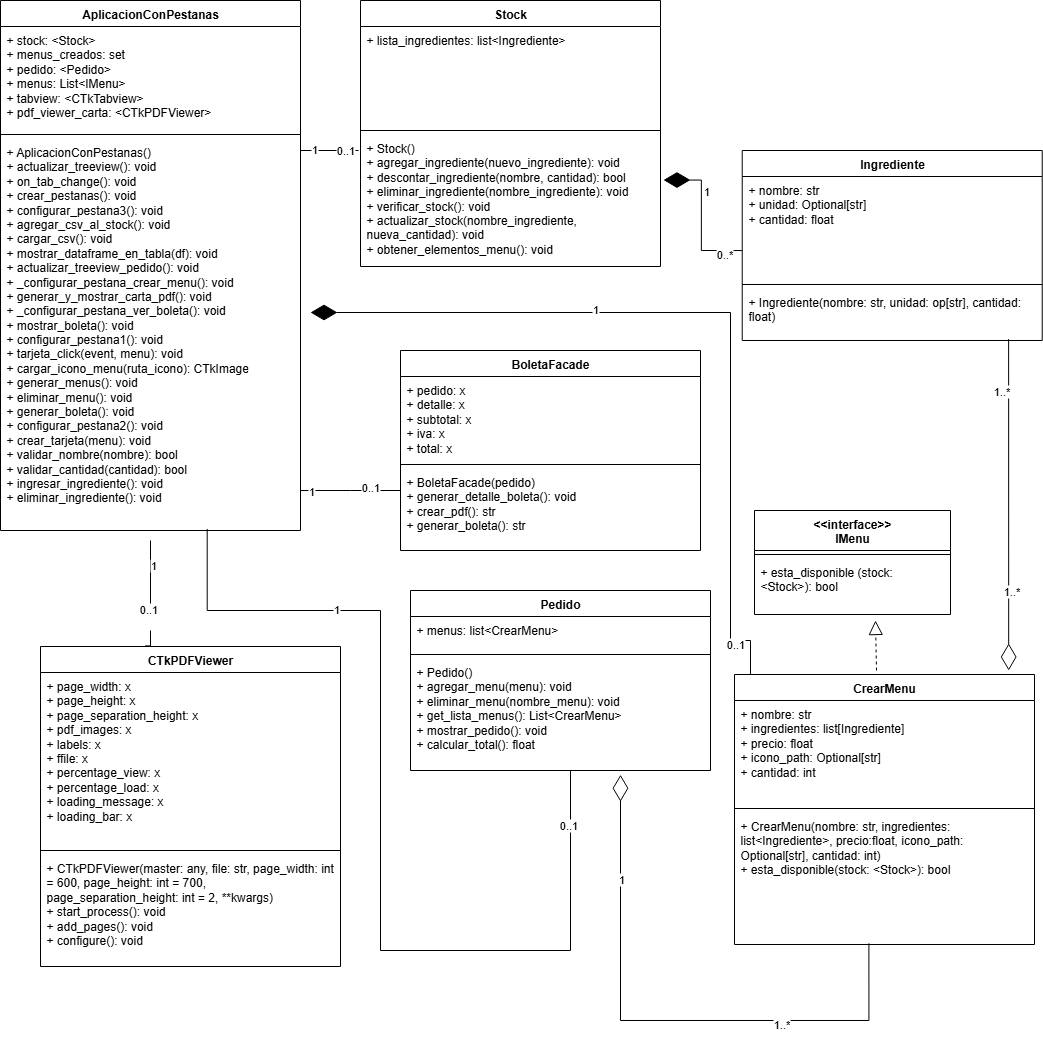
\includegraphics[width=1.1\textwidth]{Diagrama-Restaurante.drawio.png}
    \caption{Diagrama de clases de la aplicación.}.
\end{figure}



La clase \textbf{\textit{AplicacionConPestanas}} es la principal clase del programa, ya que es ella la que se usa para configurar la interfaz de CustomTkinter e instanciar, relacionar y modificar el resto de clases del sistema, las cuales se describen a continuación brevemente:
\begin{itemize}
    \item La clase \textit{Stock} es aquella donde se administra la información de ingredientes, y que servirá para determinar la disponibilidad de menúes (o platos) en función de si existen los ingredientes requeridos o no, y tiene una relación de asociación con \textit{AplicacionConPestanas}, ya que pese a que esta última instancia un objeto Stock, no hay un contenedor de los objetos instanciados (lista) y ambas clases son independientes, en la que una referencia a otra.
    \item La clase \textit{Ingrediente} es aquella que configura la información de un ingrediente en base a sus tres atributos principales y que coinciden con el estándar de información del archivo CSV. Es el elemento principal de la clase Stock.
    \item La clase \texit{CrearMenu} es donde se configura la información de un menú/platillo y se configura en base a objetos Ingredientes, debido a la relación explicada en la clase Stock. 
    \begin{itemize}
        \item[$\rightarrow$] Debido a la relación entre Stock y menúes, los objetos CrearMenu tienen una relación de agregación con los objetos Ingrediente, ya que toman ingredientes determinados y los configuran como parte de sus requisitos (los ingredientes requeridos o que forman parte de CrearMenu deben coincidir con ingredientes existentes en Stock).
        \item[$\rightarrow$] Exclusivamente, esta clase cuenta con una relación de abstracción + implementación con la clase IMenu, la cual corresponde a una interfaz que verifica que la construcción de CrearMenu cumpla los criterios solicitados.
    \end{itemize}
    \item La clase \texit{Pedido} es la clase donde se configura la información del pedido de un cliente en particular.
        \begin{itemize}
            \item[$\rightarrow$] La aplicación solo puede trabajar con máximo un Pedido a la vez, o con carencia de este, esto en una relación de asociación, ya que la existencia de ambos es bastante independiente (salvo por la instanciación que depende AplicacionConPestanas).
            \item[$\rightarrow$] La clase Pedido se configura en base a los menúes (CrearMenu) instanciados, y los va agregando en sí, teniendo la posibilidad de tener 1 o muchos menúes (de lo contrario Pedido estaría vacío y no habría datos con los que trabajar).
        \end{itemize}
    %\item La clase \texit{BoletaFacade} EDU TU PARTE
    \item La clase \textit{CtkPDFViewer} es una clase auxiliar que sirve para crear la visualización del archivo PDF con la función de carga de PDF de \textit{AplicacionConPestanas}.
\end{itemize}


\subsection{Implementaciones de codigo}

Entraremos a mas profundidad sobre el codigo nuevo o nuevas funciones que se aplicaron para la utilidad de nuestro proyecto, explicando el porque y que hacen.

\begin{lstlisting}[language=Python, caption={Implementaciones de codigo}, frame=single]
# antes
def actualizar_treeview(self):
    pass
# despues
def actualizar_treeview_stock(self):
    self.treeview_stock.delete(*self.treeview_stock.get_children())
        for ingrediente in sorted(self.stock.lista_ingredientes, key=lambda item: item.nombre):
            self.treeview_stock.insert("", "end", values=(
                ingrediente.nombre, ingrediente.unidad, ingrediente.cantidad))
\end{lstlisting}

Se rellena codigo vacio para darle una utilidad especifica a la pestaña stock porque mas adelante de implemento una funcion que se podria confundir, entonces:

\newpage

\begin{itemize}
    \item Se le da un nombre mas especifico, para no confundir.
    \item Borra completamente la tabla cada que se actualiza para evitar que se dupliquen ingredientes con \verb|self.treeview_stock.delete(...)|
    \item Se ordenan los ingredentes de forma alfabetica para una demostracion mas ordenada y profesional, con \verb|sorted(...)|
    \item Se rellena la tabla con informacion reciente obtenida por \verb|self.stock.lista_ingredientes|
\end{itemize}
Con todas estas funcionalidades se logra una funcion correcta,limpia y ordena para la pestaña stock.

\begin{lstlisting}[language=Python, caption={Implementaciones de codigo}, frame=single]
# antes
def generar_menus(self):
    pass
# despues
def generar_menus(self):
    for tarjeta in self.frame_tarjetas.winfo_children():
        tarjeta.destroy()
    listaMenus = get_default_menus()
    columna = 0
    for menu in listaMenus:
        if menu.esta_disponible(self.stock):
            columna += 1
            self.crear_tarjeta(menu, columna)
\end{lstlisting}
\textbf{Utilidades destacadas:}
\begin{itemize}
    \item \verb|for tarjeta in self.frame_tarjetas.winfo_children(): tarjeta.destroy()|es un bucle cual recorre todos los elementos que ya existen dentro de \verb|self.frame_tarjetas| y los borra para una limpieza.
    \item \begin{lstlisting}
        listaMenus = get_default_menus()
        ...
        for menu in listaMenus:
            if menu.esta_disponible(self.stock):
                ...
    \end{lstlisting}
    Esta es la mas importante del bloque ya que recorre todos los menus disponibles por el restaurante formando una lista. Para despues verificar si lo puede preparar.
    \item \begin{lstlisting}
        columna = 0
        ...
            if menu.esta_disponible(self.stock):
                columna += 1
                self.crear_tarjeta(menu, columna)
    \end{lstlisting}
    Por cada menú que SÍ está disponible, incrementa un contador \verb|(columna)| y luego llama a la función \verb|self.crear_tarjeta| para que dibuje la tarjeta en la pantalla.
\end{itemize}

\newpage

\begin{lstlisting}[language=Python, caption={Implementaciones de codigo}, frame=single]
    def ingresar_ingrediente(self):
        nombre = self.entry_nombre.get()
        unidad = self.combo_unidad.get()
        cantidad = self.entry_cantidad.get()

        if not self.validar_nombre(nombre) or not self.validar_cantidad(cantidad):
            return

        ingrediente_a_agregar = Ingrediente(nombre, unidad, float(cantidad))

        self.stock.agregar_ingrediente(ingrediente_a_agregar)

        self.entry_nombre.delete(0, 'end')
        self.entry_cantidad.delete(0, 'end')

        self.actualizar_treeview_stock()
\end{lstlisting}
Funcion importante que bien ya sabiendo por su nombre, cumple con la utilidad de que funcione el boton de \textbf{Ingresar ingrediente} en la pestaña de stock, cumpliendo con el requerimiento de que se pueda ingresar cualquier ingrediente correctamente.


\end{document}
